\chapter{Problem statement}\label{ch:problem}

%Currently there is no way of testing the full chain of devices towards, and including an application to their limits, without spending a lot of money on dedicated commercial load testing products.
Since today servers can be equipped with 40 and 100Gb/s Network Interface Cards (NICs). 
The OS and the running applications should be able to process the amount of inbound traffic from the NIC.
Network infrastructure hardware should be able to process the data from or to the NIC at line rate.
Stateful devices such as a firewall or a load balancer can be present in the path to a service. 

Testing the entire infrastructure using dedicated commercial equipment for every new service is costly.
Nikhef is constantly upgrading infrastructure devices to meet the increasing demands of bandwidth. 
Currently the engineers from Nikhef rely on the hardware specification from the vendors. 
Engineers at Nikhef have a need to find the limitations of the hardware, before they put the hardware into production. 
Budget constraints do not allow for the procurement of special commercial hardware or (expensive) tooling. 

A wide variety of tools are available to generate traffic for layer 2 and 3 testing. Nikhef is interested in TCP traffic specifically.  
Some of the tools are able to setup TCP sessions to transfer data. 
%But what tool is best used for specific application testing?   
Nikhef wants the ability to test hardware they might buy up to the OSI application layer (layer 7) if applicable. 
Until now they are not able to go beyond the transport layer (layer 4).
Figure \ref{fig:layeredtesting} provides a representation of testing at different OSI layers.
Testing at these layer can reveal different limitations from the infrastructure.

\begin{figure}[H]
  \includegraphics[scale=0.5]{images/layered-tests.pdf}
  \caption{Representation of the mentioned OSI layers in a network diagram.}
  \label{fig:layeredtesting}
\end{figure}

\section{The reliability of TCP}\label{sec:sessionbased}
When sending data over UDP, data gets generated and transported to the destination without any form of reliability. 
If the destination UDP port is open the data will be forwarded to the application listening on that specific port.
When the destination does not listen on that specific UDP port the data will be dropped.
The protocol does not provide feedback for any of the actions taken at the receivers side (except for ICMP error messages).
 
In contrast to UDP, TCP guarantees the delivery of the data as long as the session is established between the end nodes.
The session needs to be created before data can be exchanged. 
A three way handshake between source and destination is performed in order to synchronize TCP settings. 
Guaranteed delivery is realized by acknowledging received data and resending unacknowledged data. 
Other techniques like flow control, congestion control and fast retransmission of packets ensure that data is delivered in time and offered to the higher layer protocol in the correct order. 
These techniques all require resource reservation at the client and the server, and at stateful network devices along the path between client and server. 

The techniques implemented in TCP require buffers to store data until the data is acknowledged by the receiving end.
The buffer sizes are reserved by the OS per session and are negotiated during the three way handshake.  
When the amount of new sessions is higher than the amount of sessions that get closed due to a time-out or by terminating the session, server resources are depleted.

When it comes to layer 7 protocols like HTTP, more resources need to be reserved. HTTP sessions, HTTP state and application state need to be saved. 
HTTP requests need to be processed, a response needs to be generated and sent over the session to the user. Normally a web server will cache files that are requested for a specific time using up valuable memory. Hosting a dynamic web page requires the web server to generate the page on request which makes the CPU utilization higher than just hosting static web content. 

\section{Assumptions and constraints}\label{sec:specifications}
In order to execute some experiments and interpret their results, specific technical constraints in the real world operating environment and several key implementation parameters are important for this research.

\paragraph{Overloading}\label{par:overload}\mbox{}\\
All the built in techniques used by TCP ensure an IP path will not be overloaded with congestion. 
In order to find the weakest link in the path towards a service, data should be sent using the expected maximum capacity of the devices in the path.
When client and server are connected with 40Gb/s interfaces one should send data using the full capacity of the links.
This could result in overloading a device in the path, which immediately shows that the intermediate device is the weakest link.

When data can be sent at the link's full capacity, there might be other hardware limitation (maximum amount of packets per second or a maximum amount of session per second) in the path to the destination.
For systems administrators it is important to know these limitation for monitoring purposes.

\paragraph{Throughput}\label{par:throughput}\mbox{}\\
The increasing need for bandwidth requires high capacity links between clients and destination in order to minimize transfer times.
A link's throughput is the most significant value for generating load. 
This research considers links with a capacity of 40Gb/s and up, as high bandwidth link's.
Therefore considered tools need to generate at least 40Gb/s of bandwidth, this is the first requirement.  

%When using TCP the header causes 12 bytes more overhead in comparison to a UDP header (a UDP header is 8 bytes). But in return TCP offers techniques that will not overload a device. 

\paragraph{Frame size}\label{par:packetsize}\mbox{}\\
Ethernet is used during this research, therefore all references to frame sizes are based on Ethernet standards\cite{ethernet_frame_2017} with IP and TCP headers included.
Due to collision detection the minimum payload inside an Ethernet frame is 46 bytes.
The Ethernet frame and the payload combined have a minimum size of 64 bytes. 
A VLAN tag is excluded which adds 4 bytes.
A packet is always preceded with a 8 byte preamble.
A 12 byte Inter Frame Gap between frames is used to separate the frames. 
This makes a total of at least 88 bytes of data from the beginning of a packet to the beginning of a new packet. 
A representation of an Ethernet frame that is used in the report is given in figure \ref{fig:juniperethernetframe}. 

\begin{figure}[H]
  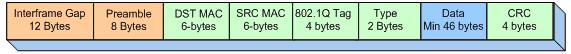
\includegraphics[scale=1]{images/ethernetframe.jpg}
  \caption{Representation of an Ethernet frame used during this report.}
  \label{fig:juniperethernetframe}
\end{figure}

\paragraph{Packets per second}\label{par:pps}\mbox{}\\
When a link has a capacity of 40Gb/s and packets have a minimum size of 88bytes (which includes the inter frame gap, the preamble, the data link frame and a VLAN tag) a maximum of 56.8 million packets per second (Mpps) can be transferred over the link in one direction. When using a 100Gb/s line the theoretical maximum is 142 Mpps.   
The research is focusing on 40Gb/s links and therefore the second requirement is that a tool needs to be able to generate 56.8 million packets per second in order to be considered for the proposed tests.

\paragraph{Sessions}\label{par:sessions}\mbox{}\\
A TCP session is a unique tuple of source IP, destination IP, source port and destination port. 
An established session may be used to send more than one packet and is to transfer data bidirectional.
The amount of sessions per second is a determining factor for the availability of services behind stateful devices. 
A firewall, for example, needs to keep track of the states of the sessions from source to destination. 
When new sessions to a server are opened, the firewall has to process them according to the rule base. 
When a session is approved, most firewall vendors move it to fast-path processing. 
This is a table with accepted sessions, allowing traffic in the same session to be handled in hardware. This means that only the first packet of a new session is handled in the slow-path and the limitations of a firewall can be found in the amount of new sessions per second.
The amount of sessions the tool is capable of generating is the third requirement for this research focuses on during the experimental phase.

\paragraph{Application specific traffic}\mbox{} \\
According to Sandvine\cite{phenomena_2017},a global communications solutions service provider that published bi-annual traffic baseline reports, around 70\% of the traffic on the Internet is streaming audio and video. 
Dynamic Adaptive Streaming over HTTP (DASH)\cite{dash} is used to stream video and audio over HTTP. 
Netflix uses DASH to deliver content to the users. 
Next to DASH, streaming video services like YouTube are also accessible over HTTP.
This makes HTTP a suited protocol to use for layer 7 tests during the research.  

\paragraph{Packet size}\label{par:packetsize}\mbox{}\\
According to Murray et all. \cite{murray2012state}  in 2012, 99\% of the traffic inside a corporate network has an MTU size of maximum 1500 bytes. 
When using Jumbo frames\cite{alliance_2017} (best practice is an MTU of 9000 bytes towards clients\cite{jet}) the amount of overhead is less because more data can fit in one packet. 
More data inside a packet could results in less packets. 
Jumbo packets are helpful when large amounts of data need to be transfered between 2 nodes.  
Jumbo packets are not used during the project because according to Murray et all. less than one percent of transferred data has an MTU larger than 1500 bytes. 
Exceptions can be made during a test to see if hardware limits can be reached.

\paragraph{End-to-end testing}\label{par:endtoend}\mbox{}\\
Testing only bandwidth between two links does not test the limitations of an application. The application and the kernel should be tested using OSI layers above layer 4. 
When an application is connected with a 40Gb/s link, it does not mean that the application can process 40Gb/s. 
End-to-end testing is a term used in this report to refer to tests that are application based.
A client sending application layer protocol requests en the server responding with application layer protocol requests.  

\section{Research question}\label{sec:researchquestion}
The problem statement and the specifications lead to the following research question.

\begin{center}
\textit{What are the requirements to perform high bandwidth session based throughput testing and how can this be applied to end-to-end application level testing?} \\
\end{center}

